%====================================================================================
\section[Provisión de Bn Público]{Provisión óptima de un Bien Público}
%====================================================================================

\begin{frame}{Provisión óptima de un Bien Público}
	Cuando
		$$\left| RMS_A\right| + \left| RMS_B\right| = TMT = CM(G)$$
	el cual equivale a:
		$$\sum DAP = CMg$$
	Es posible que un determinado bien público sea valorado de manera distinta por cada consumidor.\\
	Entonces, ¿cuánto están dispuestos a pagar por tener el bien?
		\begin{itemize}
			\item DAP, o
			\item Precios de reserva
		\end{itemize}
\end{frame}
%------------------------------------------------
\begin{frame}{Precios de Reserva}
	\begin{itemize}
		\item El precio de reserva de un consumidor por unidad de un bien es su máxima disposición a pagar por él. 
		\item Sea w La riqueza de un consumidor. 
		\item La utilidad de no tener el bien se puede expresar como
			$$U(w,0)$$
		\item La utilidad de consumir una unidad del bien, pagando $p$, es
			$$U(w - p, 1)$$
		\item El precio de reserva r es definido por
			$$U(w,0) = U(w-r, 1)$$
	\end{itemize}
\end{frame}
%------------------------------------------------
\begin{frame}{¿Cuando debe ser suministrado un bien Público?}
	Una unidad del bien público cuesta $c$ unidades monetarias. Se tiene dos consumidores, $A$ y $B$. Los pagos individuales para la provisión del bien público son $g_A$ y $g_B$. Si $g_A + g_B \geq c$  el bien es suministrado.
	\begin{itemize}
		\item Los pagos (aportes) deben ser racionalmente individuales; es decir
			\begin{gather*}
				U_A(w_A,0) \leq U_A(w_A - g_A,1)
				\intertext{y}
				U_B(w_B,0) \leq U_B(w_B - g_B,1)
			\end{gather*}
			Por lo tanto, necesariamente
				$$g_A \leq r_A \quad \text{y} \quad g_B \leq r_B$$
	\end{itemize}
\end{frame}
%------------------------------------------------
\begin{frame}{¿Cuando debe ser suministrado un bien Público?}
	\begin{itemize}
		\item Y si
				\begin{gather*}
					U_A(w_A,0) < U_A(w_A - g_A,1)
					\intertext{y}
					U_B(w_B,0) < U_B(w_B - g_B,1)
				\end{gather*}
			entonces hay una mejora paretiana de ofrecer una unidad de bien público, por tanto, es suficiente 
			que
				$$r_A + r_B > c$$
			para que sea eficiente suministrar el bien público.
	\end{itemize}
\end{frame}
%------------------------------------------------
\begin{frame}{¿Provisión privada de un Bien Público?}
	\begin{itemize}
		\item Supongamos que 
			$$r_A > c \quad \text{y} \quad r_B < c$$
		Entonces $A$ ofrecería pagar por el bien aun si $B$ no hiciera su contribución. $B$ entonces disfruta del bien libremente. Es un parásito o gorrón.
		
		\item Supongamos que 
			$$r_A < c \quad \text{y} \quad r_B < c$$
		Entonces ni A ni B ofrecen pagar por el bien individualmente. Solo si $r_A + r_B > c$ es una mejora de Pareto ofrecer el bien.
	\end{itemize}
\end{frame}
%------------------------------------------------
\begin{frame}{Diferentes niveles de Bien Público}
	Un primer tipo de decisión es suministrar o no el bien público. Otro tipo de problema es decidir en qué cantidad suministrarlo.
		\begin{itemize}
			\item Sea $c(G)$ el costo de producción de $G$ unidades de bien público.
			\item Se tiene dos individuos, $A$ y $B$.
			\item El consumo privado de cada individuo será $x_A$, $x_B$.
			\item Las asignaciones presupuestales deben satisfacer
				$$x_A + x_B + x(G) = w_A + w_B$$
		\end{itemize}
\end{frame}
%------------------------------------------------
\begin{frame}{Diferentes niveles de Bien Público}
	\begin{itemize}
		\item $RMS_A \& RMS_B$ son las tasas marginales de sustitución de  $A \& B$ entre los bienes privado y  público.
		\item La condición de Pareto eficiente para ofrecer un bine público es
			$$\left| RMS_A\right| + \left| RMS_B\right| = CM(G)$$
		donde
			$$\frac{\delta x_1}{\delta G} + \frac{\delta x_2}{\delta G} = \frac{UM_G}{UM_1} + \frac{UM_G}{UM_2}$$
		$CM_G$ = costo marginal de suministrar una unidad adicional de bien público.
	\end{itemize}
\end{frame}
%------------------------------------------------
\begin{frame}{Diferentes niveles de Bien Público}
	¿Por qué la condición de Pareto eficiente es
		$$\left| RMS_A\right| + \left| RMS_B\right| = CM(G)$$
	Recordemos que el bien público es no rival en consumo; por tanto una unidad extra de bien público es totalmente consumido tanto por $A$ como por $B$.\\
	
	Supongamos que: $\left| RMS_A\right| + \left| RMS_B\right| < CM(G)$
		\begin{itemize}
			\item La $RMS$ de $A$ es la compensación que preserva su utilidad, en unidades del bien privado, por la reducción de una unidad de bien público. Similarmente se interpreta la $RMS$ para $B$.
			\item $\left| RMS_A\right| + \left| RMS_B\right|$ es el pago total a  $A \& B$ en bien privado para preservar ambas utilidades si  G es reducido en una unidad.
			\item Dado que $\left| RMS_A\right| + \left| RMS_B\right| < CM(G)$ implica que una unidad menos de bien público genera mayor cantidad de bien privado de lo que la compensación requiere.
		\end{itemize}
\end{frame}
%------------------------------------------------
\begin{frame}{Diferentes niveles de Bien Público}
		\begin{itemize}
			\item Hay un excedente que puede repartirse entre $A$ y $B$, mejorando el bienestar de ambos.
			\item Hay una mejora de Pareto al reducir $G$.
		\end{itemize}
	Ahora supongamos que $\left| RMS_A\right| + \left| RMS_B\right| > CM(G)$
		\begin{itemize}
			\item Puede aumentar la cantidad de $G$ para  mejorar el bienestar de ambos individuos.
			\item Entonces: hay una mejora paretiana de aumentar $G$.
		\end{itemize}
	Por tanto, necesariamente la producción eficiente de bien público requiere:
		$$\left| RMS_A\right| + \left| RMS_B\right| = CM(G)$$
	Y si hay n consumidores:
		$$\sum_{i=1}^{n}\left| RMS_i\right| = CM(G)$$
\end{frame}
%------------------------------------------------
\begin{frame}{Provisión privada de bienes públicos}
	\begin{itemize}
		\item Dado que los bienes públicos pueden ser compartidos en el consumo, cada consumidor tiene un incentivo para confiar en que otros consumidores adquirirán el bien público. 
		\item Esa confianza en lo que harán otros consumidores, es llamada el  comportamiento tipo gorrón o parásito.
		\item Esto conduce a la ineficiencia, porque se proveerá una pequeña cantidad del bien público.
		\item Todos los consumidores se beneficiarán con una  mayor  provisión del bien público.
	\end{itemize}
\end{frame}
%------------------------------------------------
\begin{frame}{Provisión privada de bienes públicos}
	\begin{itemize}
		\item Consideremos dos consumidores que asignan sus ingresos entre un bien privado y un bien público.
		\item Los consumidores toman los precios como dados. 
		\item Cada consumidor obtiene un beneficio de la provisión del otro.
		\item Esto introduce una interacción estratégica en los procesos de decisión.
		\item Puede encontrarse el equilibrio Nash.
	\end{itemize}
\end{frame}
%------------------------------------------------
\begin{frame}{Provisión privada de bienes públicos}
	\begin{itemize}
		\item Esta interacción es capturada en las preferencias del consumidor  h, cuya función de utilidad es
				$$U^h(x^h, g^1 + g^2)$$
		\item $x^h$= compra del bien privado, gh compra del bien público, $G=g^1+g^2$.
		\item Cada consumidor decide, considerando como dato la compra del otro consumidor.
			\begin{itemize}
				\item El consumidor 1 escoge $g^1$, para maximizar su utilidad, dado $g^2$. 
				\item El consumidor 2 escoge $g^2$, para maximizar su utilidad, dado $g^1$. 
			\end{itemize}
	\end{itemize}
\end{frame}
%------------------------------------------------
\begin{frame}{Provisión privada de bienes públicos}
	\begin{itemize}
		\item La elección del consumidor 1 es la mejor reacción a $g^2$; la elección del consumidor 2 es la mejor reacción a $g^1$.
		\item Puede analizarse las preferencias individuales respecto a diferentes combinaciones de $g^1$, $g^2$.
		\item Asumiendo que el precio de ambos bienes es 1, la elección debe satisfacer la restricción presupuestaria:
				$$M^h = x^h + g^h$$
		\item Consideremos el consumidor 1. Usando su restricción presupuestal su función de utilidad es
				$$U^1\left( M^1 - g^1, g^1 + g^2\right)$$
	\end{itemize}
\end{frame}
%------------------------------------------------
\begin{frame}{Provisión privada de bienes públicos}
	$$U^1\left( x^1, g^1 + g^2\right)$$
		\begin{itemize}
			\item Usando su restricción presupuestal: $U^1\left( M^1 - g^1, g^1 + g^2\right)$
			\item Diferenciando totalmente
					\begin{gather*}
						dU^1 = -\frac{\partial U^1}{\partial x^1}dg^1+\frac{\partial U^1}{\partial G}g^1 + \frac{\partial U^1}{\partial G}dg^2 = 0\\[0.3cm]
						-\frac{dg^2}{dg^1} = \frac{\frac{\partial U^1}{\partial x^1} - \frac{\partial U^1}{\partial G}}{\frac{\partial U^1}{\partial G}}
					\end{gather*}
			\item Las curvas de indiferencia pueden trazarse usando la tasa a la cual $g^2$ puede ser intercambiada por g1, manteniendo constante la utilidad:
					$$\left. \frac{dg^2}{dg^1}\right|_{U^1 cte} = \frac{\frac{\partial U^1}{\partial x^1} - \frac{\partial U^1}{\partial G}}{\frac{\partial U^1}{\partial G}}$$
		\end{itemize}
\end{frame}
%------------------------------------------------
\begin{frame}{Provisión privada de bienes públicos}
	Dado $\bar{g}^2$, la mejor respuesta del consumidor 1 se da cuando la pendeinte es nula, esto es:
		$$\frac{\partial U^1}{\partial x^1} = \frac{\partial U^1}{\partial G} \rightarrow g^1 = \hat{g}^1$$
	Antes de dicho punto, la pendiente es negativa:
		$$\frac{\partial U^1}{\partial x^1} < \frac{\partial U^1}{\partial G} \rightarrow g^1 < \hat{g}^1$$
\end{frame}
%------------------------------------------------
\begin{frame}{Provisión privada de bienes públicos}
	Después de dicho punto, la pendiente es positiva:
		$$\frac{\partial U^1}{\partial x^1} > \frac{\partial U^1}{\partial G} \rightarrow g^1 > \hat{g}^1$$
	Variando la provisión del consumidor 2, se obtiene el locus de decisiones del consumidor 1= mejor reacción del consumidor 1
	
		\begin{center}
			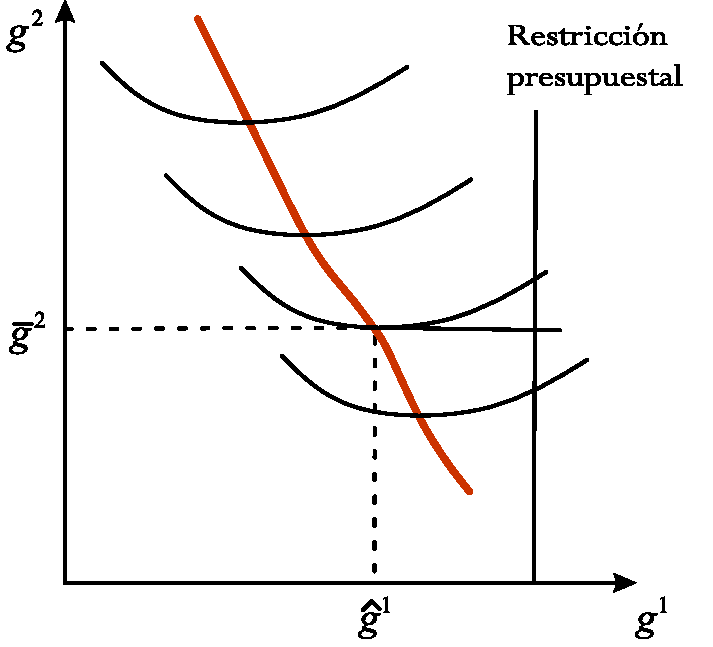
\includegraphics[width = 0.52\linewidth]{figures/fig_08.pdf}
		\end{center}
\end{frame}
%------------------------------------------------
\begin{frame}{Provisión privada de bienes públicos}
	Similarmente se obtiene la curva de reacción del consumidor 2.
		\begin{center}
			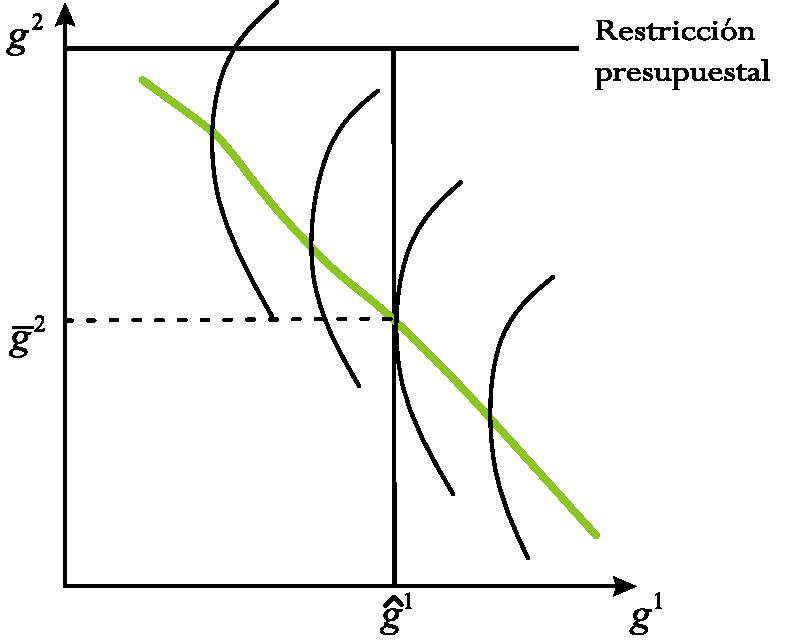
\includegraphics[width = 0.8\linewidth]{figures/fig_09.pdf}
		\end{center}
\end{frame}
%------------------------------------------------
\begin{frame}{Provisión privada de bienes públicos}
	\begin{itemize}
		\item El equilibrio Nash es donde las elecciones de ambos consumidores son las mejores reacciones al otro.
		\item Nadie tiene incentivo a cambiar su elección.
		\item Esto ocurre donde se cruzan las funciones de mejor respuesta.
		\item Las elecciones de equilibrio son: $\hat{g}^1$ y $\hat{g}^2$
	\end{itemize}

	\begin{center}
		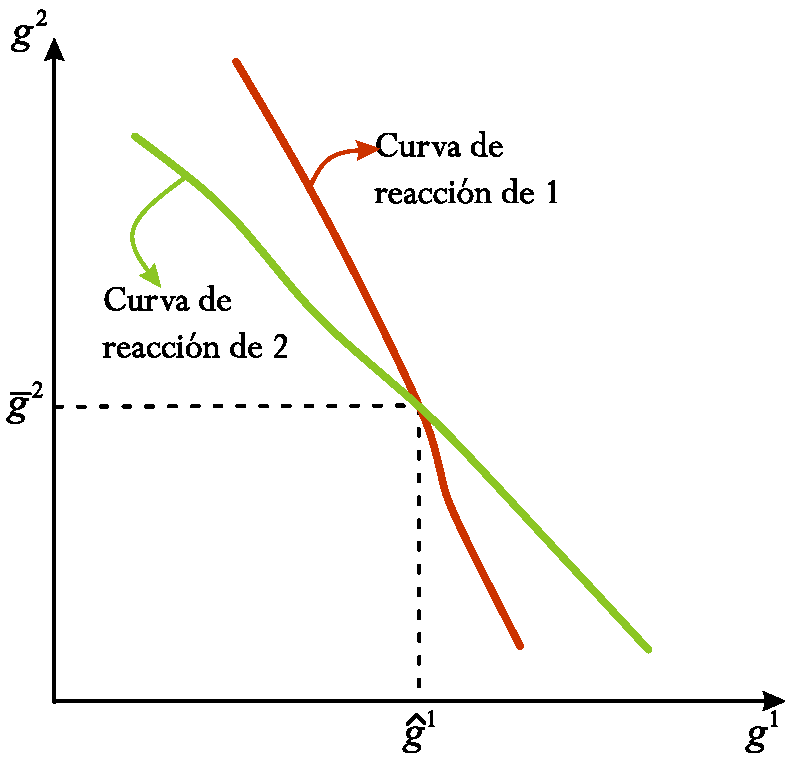
\includegraphics[width = 0.52\linewidth]{figures/fig_10.pdf}
	\end{center}
\end{frame}
%------------------------------------------------
\begin{frame}{Provisión privada de bienes públicos}
	\begin{itemize}
		\item La provisión privada de equilibrio es ineficiente.
		\item Pero es racional desde el punto de vista privado. 
		\item Un incremento simultáneo en la provisión de ambos consumidores proporciona una mejora de Pareto.
		\item Las asignaciones  Pareto-eficientes son los puntos de tangencia de las curvas indiferencia.
	\end{itemize}

	\begin{center}
		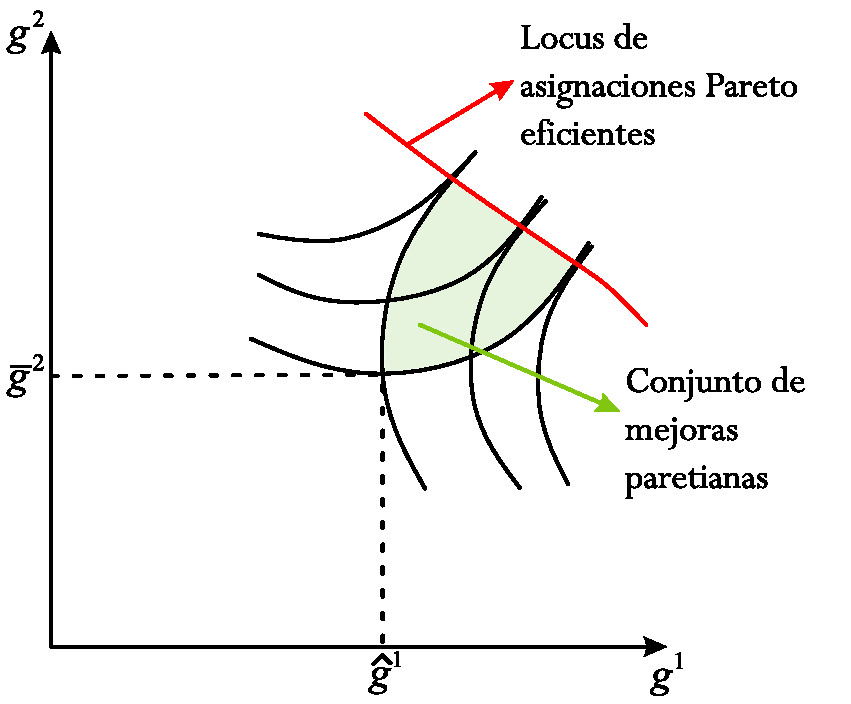
\includegraphics[width = 0.57\linewidth]{figures/fig_11.pdf}
	\end{center}
\end{frame}
%------------------------------------------------
\begin{frame}{Provisión eficiente}
	\begin{itemize}
		\item En la asignación Pareto-eficiente las curvas de indiferencia son tangentes.
		\item Esto no implica igualar las TMS porque las curvas de indiferencia son definidas sobre cantidades de bien público consumidas por los dos consumidores.
		\item La condición de eficiencia implica la suma de las TMS.
		\item La condición de tangencia es
				$$\left. \frac{dg^2}{dg^1}\right|_{U^1 cte} = \left. \frac{dg^2}{dg^1}\right|_{U^2 cte}$$
		\item Para el consumidor 1 ya hallamos que:
				$$\left. \frac{dg^2}{dg^1}\right|_{U^1 cte} = \frac{\frac{\partial U^1}{\partial x^1} - \frac{\partial U^1}{\partial G}}{\frac{\partial U^1}{\partial G}}$$
	\end{itemize}
\end{frame}
%------------------------------------------------
\begin{frame}{Provisión privada de bienes públicos}
	Similarmente para el consumidor 2:
		$$U^2\left( x^2, g^1 + g^2\right)$$
			\begin{itemize}
				\item Usando su restricción presupuestal: $U^2\left( M^2 - g^2, g^1 + g^2\right)$
				\item Diferenciando totalmente
				\begin{gather*}
					dU^2 = -\frac{\partial U^2}{\partial x^2}dg^1+\frac{\partial U^2}{\partial G}g^1 + \frac{\partial U^2}{\partial G}dg^2 = 0\\[0.3cm]
					\frac{dg^2}{dg^1} = \frac{\frac{\partial U^2}{\partial G}}{\frac{\partial U^2}{\partial x^2} - \frac{\partial U^2}{\partial G}}
				\end{gather*}
			\end{itemize}
\end{frame}
%------------------------------------------------
\begin{frame}{Provisión eficiente}
	Entonces
		$$\left. \frac{dg^2}{dg^1}\right|_{U^1 cte} = \left. \frac{dg^2}{dg^1}\right|_{U^2 cte}$$
	Implica que:
		\begin{gather}
			\frac{\frac{\partial U^1}{\partial x^1} - \frac{\partial U^1}{\partial G}}{\frac{\partial U^1}{\partial G}} = \frac{\frac{\partial U^2}{\partial G}}{\frac{\partial U^2}{\partial x^2} - \frac{\partial U^2}{\partial G}} \label{eq1}
		\end{gather}
	Definamos $TMS$:
		$$TMS_{G,x}^{h} \equiv \frac{\partial U^h/\partial G}{\partial U^h/\partial x^h}$$
	Multiplicando y diviendo (\ref{eq1}), a la izquierda por $\frac{1}{\partial U^1/\partial x^1}$ y a la derecha por $\frac{2}{\partial U^2/\partial x2}$ se obtiene:
		$$\frac{1 - TMS_{G,x}^1}{TMS_{G,x}^1} = \frac{TMS_{G,x}^2}{1-TMS_{G,x}^2}$$
\end{frame}
%------------------------------------------------
\begin{frame}{Provisión eficiente}
	Operando:
		\begin{gather*}
			\frac{1 - TMS_{G,x}^1}{TMS_{G,x}^1} = \frac{TMS_{G,x}^2}{1-TMS_{G,x}^2}\\
			1 - TMS_{G,x}^2 - TMS_{G,x}^1 + TMS_{G,x}^1 \times TMS_{G,x}^2 = TMS_{G,x}^1 \times TMS_{G,x}^2
		\end{gather*}
	Volvemos a la  Regla de Samuelson:
		$$TMS_{G,x}^1 \times TMS_{G,x}^2 = 1$$
	\begin{itemize}
		\item La suma de las tasas marginales de sustitución es igualada a la tasa marginal de transformación entre bienes público y privado.
		\item La tasa marginal de sustitución mide el beneficio marginal para un consumidor de una unidad adicional de bien púbico.
		\item La tasa marginal de transformación es el costo marginal de otra unidad.
	\end{itemize}
\end{frame}